\subsection{OP5 comparison field: sampled multimode geometry}
\label{subsec:op5-multimode-slices}

This figure records the original affine baseline of 29 October 2026.
Later quadratic fits are discussed separately in
Section~\ref{subsec:v410-field-compatibility}; they do not replace these data.
As a diagnostic in the declared classical comparison sector, consider a sum
of two exponential modes with independent affine complex spinor amplitudes.
A common positive amplitude factor enforces the necessary scalar condition
\(h\Psi^\dagger(Z\otimes\beta)\Psi=8\), where
\(Z=\operatorname{diag}(1,-1,0)\). This condition does not replace the full
probe equation. The coframe and its inverse are recomputed from the fields;
the original comparison couplings and zero Lorentz spin connection are
retained. This is not an identification of the induced Levi--Civita connection.

Figure~\ref{fig:op5-multimode-slices} evaluates one saved approximate field,
without refitting, on all six coordinate-plane cuts through
\((t,x,y,z)=(1,0.6,0,0)\). Each cut uses nine positions per axis with offsets
\(\pm0.01\) in comparison coordinates. These are six overlapping
\(9\times9\) slices, not a full four-dimensional grid.
The largest sampled residual norm is approximately \(0.03868\), the smallest
absolute coframe determinant is \(9.6991\), and every sampled \(g^{00}\)
is negative. These are finite-sample diagnostics, not uniform bounds.

For the frame images \(E_i\) and \(E_j\) of coordinate directions, the
oriented area is represented by the full bivector \(E_i\wedge E_j\).
Its signed squared area is \(g_{ii}g_{jj}-g_{ij}^{2}\). The spatial cross
product of their spatial projections supplies the spatial bivector components;
time--space components must also be retained. Neither this area nor a mixed
metric component alone establishes Riemann curvature.

The explicit smooth field makes mixed derivatives consistent wherever its
normalization is regular, but its nonzero equation residual remains.
No exact regional solution, native action derivation, or OP5 closure is claimed.
The numerical record and reproduction files are archived under
\texttt{analysis/op5-field-slices/}.

\begin{figure}[p]
\centering
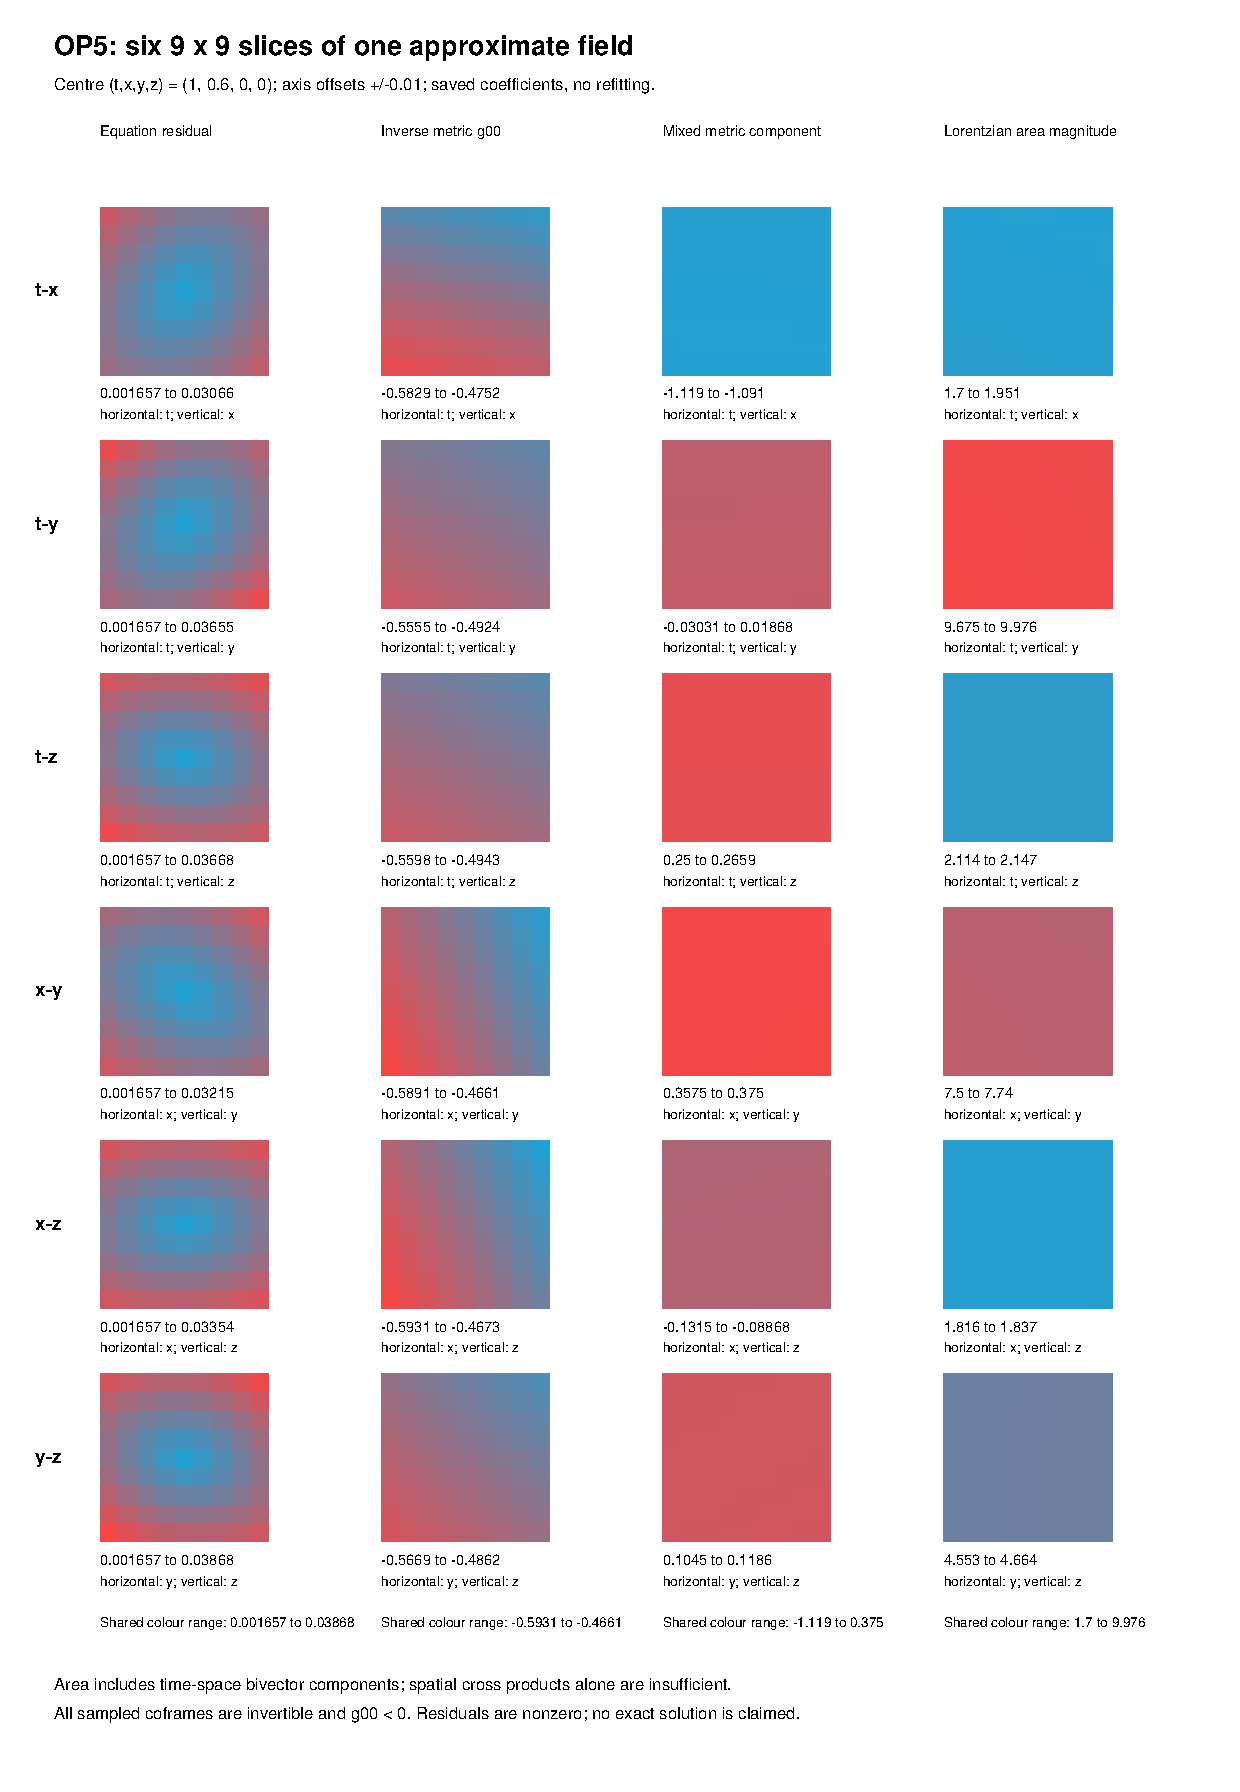
\includegraphics[width=\textwidth,height=0.78\textheight,keepaspectratio]{figures/op5-slices-9x9.pdf}
\caption{Original affine baseline: six \(9\times9\) cuts of the same approximate OP5 comparison field.
Columns show the full probe-equation residual norm, \(g^{00}\), the normalized
mixed metric component \(g_{ij}/\sqrt{|g_{ii}g_{jj}|}\), and the Lorentzian
area magnitude \(\sqrt{|g_{ii}g_{jj}-g_{ij}^{2}|}\). A common colour range is
used within each column; local numerical ranges appear below each panel.
Horizontal and vertical coordinates are identified per panel.
Invertibility and spacelike constant-\(t\) cuts hold at the sampled points;
the residual is nonzero.}
\label{fig:op5-multimode-slices}
\end{figure}
